% !TeX root = ../thuthesis-example.tex

\chapter{分段对称模式挖掘算法}
第3章介绍了全局对称模式挖掘算法,
然而,真实的对称模式往往是聚合在一条
长时间序列之中的,其中有缺失点、异常点、噪声点等种种干扰,
而且多个对称子序列可能相互重叠在一起,
使得分段对称模式挖掘和结果判断更加困难。
因此,本节设计了一种从长时间序列中挖掘出分段对称模式的算法,
并根据Apache IoTDB的存储和计算方式
对分段对称模式挖掘算法进行了优化。

本章的组织结构如下所示,
4.1节基于分段长度约束$w$,设计了一种计算所有长度
为$w$的时间子序列对称度的算法;4.2节介绍了根据
时间序列数据特征和对称度分布确定对称度阈值的算法;
4.3节根据贪心策略和对称度阈值挖掘出所有的对称模式;
4.4节分析了基于IoTDB数据库实现分段对称模式挖掘算法
的两种方式,并对比了这两种方式的优劣和适用场景。

\section{分段时间序列对称性度量算法}
要对时序数据进行对称子序列的挖掘,首先要做的就是把时间序列划分成
一段一段的子序列,然后对子序列进行对称度度量。
时间序列断点检测算法是一种经典的时间子序列划分方法。
图~\ref{fig:break_detection}展示了时间序列断点检测算法的计算流程。
为了检测时间序列中的关键点,该算法采用直线对整体的时间序列数据
进行拟合,如果时序数据的趋势发生了变化,则用多条直线拟合整条
时序数据。该算法使用单变量线性回归模型拟合每段时间
序列,每处理一个新数据点就重新计算多段拟合误差,利用动态规划算法
全局最大化分段效果。时间序列断点检测算法的好处是可以根据时间序列
的趋势进行关键点的判断,但是,工业时间序列中的对称模式多种多样,
除去首尾点之外,模式内部可能也存在关键点,只识别出关键点无法成功
分割出对称模式。此外,时间序列断点检测算法的复杂度高达
$O\left(n^{3}\right)$,甚至超出了对称模式挖掘算法的复杂度,
在实际工业场景中不具备应用价值。
\begin{figure}[t]
  \centering
  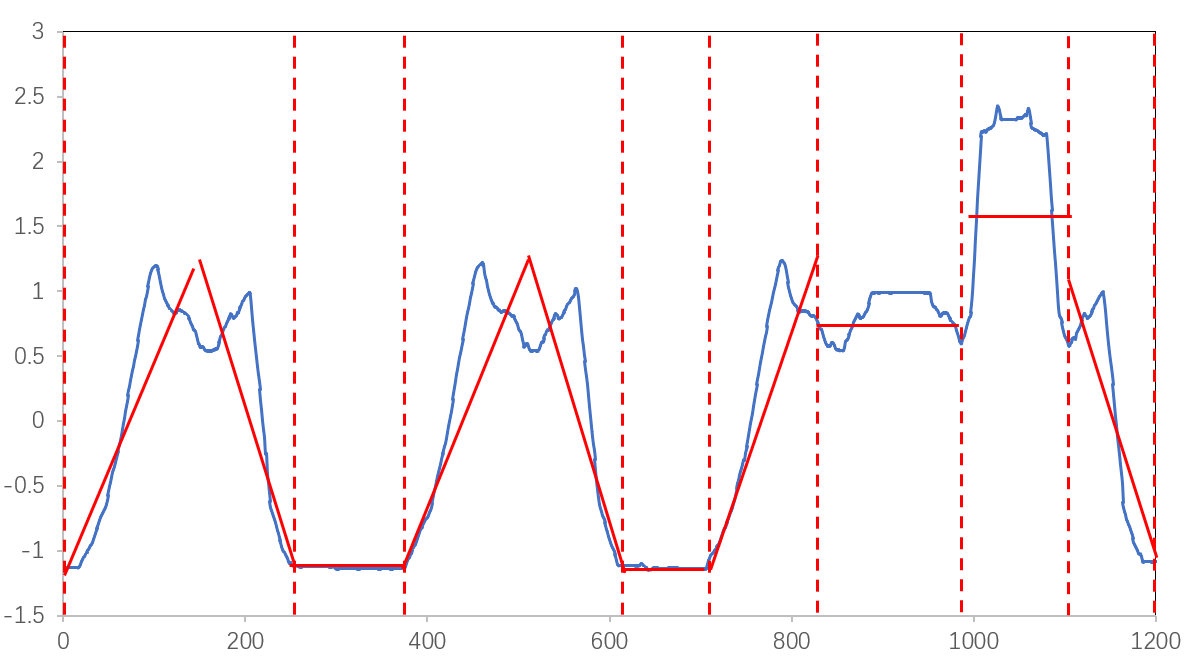
\includegraphics[width=0.66\linewidth]{break_detection.png}
  \caption{时间序列断点检测与直线拟合图}
  \label{fig:break_detection}
\end{figure}

基于此,本文选择基于滑动窗口的时间序列分段算法。滑动窗口源于网络流量控制
技术,在时间序列分析领域可以用于在特定窗口大小的子序列上执行对称度计算的
操作。通过维护一个不断向前滑动的窗口,划分出全部的时间序列分段。
图~\ref{fig:sliding_window}展示了使用滑动窗口将时间序列中每个长度为$w$的子序列划分出来的过程。

\begin{figure}[h]
  \centering
  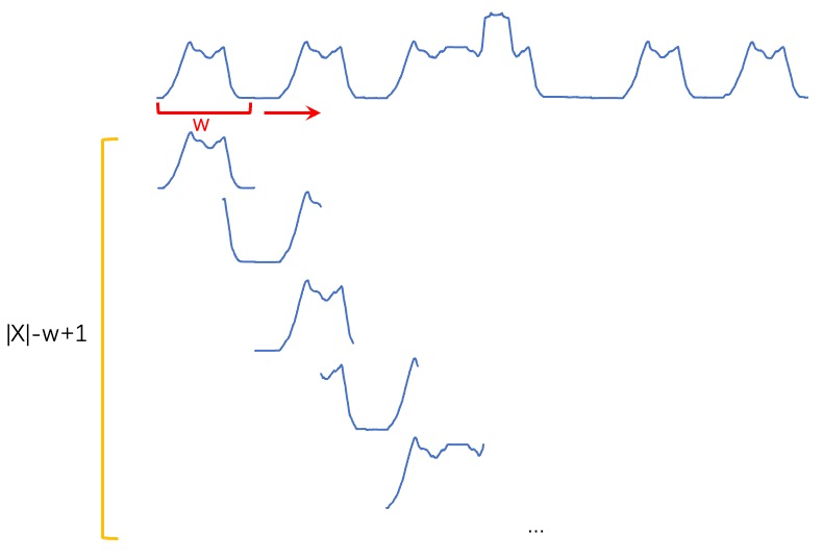
\includegraphics[width=0.66\linewidth]{sliding_window.png}
  \caption{滑动窗口时间序列分段示例}
  \label{fig:sliding_window}
\end{figure}

在滑动窗口模型中,可以直接使用3.1节所述的全局对称性度量算法计算每段时间子序列
的对称性,由于单个时间序列对称性计算的时间复杂度为$O(w^2 )$,所以全部
分段时间序列对称性度量算法的时间复杂度为$O\left(|X| \times w^{2}\right)$。
然而,利用滑动窗口和区间动态规划算法的特点可以将复杂度降低一个阶数。
考虑时间序列$X$两段长度为$w$的连续子序列$S_{i}=\left(\left(t_{i}, x_{i}\right),\left(t_{i+1}, x_{i+1}\right), \dots,\left(t_{i+w-1}, x_{i+w-1}\right)\right)$
和$S_{i+1}=\left(\left(t_{i+1}, x_{i+1}\right),\left(t_{i+2}, x_{i+2}\right), \dots,\left(t_{i+w}, x_{i+w}\right)\right)$的对称度度量,
根据式~\ref{eq:dp_item}的状态方程,时间子序列$S_i$的对称度
$D P(i, i+w-1)$由$DP(i,i+w-2)$,$DP(i+1,i+w-1)$和$DP(i+1,i+w-2)$
的最小值推导而来,而子序列$S_{i+1}$的对称度$D P(i+1, i+w)$由
$D P(i+1, i+w-1)$,$DP(i+2,i+w)$和$DP(i+2,i+w-1)$的最小值推导
而来,这两个对称度的计算都使用到了状态$DP(i+1,i+w-1)$,如果分别计算
将会产生大量的重复计算。然而,考虑到动态规划方程的无后效性,如果先计算
出时间序列$X$中所有长度为$w-1$和$w-2$的子序列对称度并保存下来,
则$S_i$和$S_{i+1}$的状态可以直接计算得到。
图~\ref{fig:fregment}展示了分段时间序列对称度推导过程,
假设时间序列$X$的长度为9,子序列长度即滑动窗口长度为5,采用窗口长度由小到大的
自底向上的推导顺序,每段子序列对称度状态都可以通过$O(1)$的复杂度计算得到,最终所有时间子序列
对称度度量的复杂度由状态个数决定,最底层长度为1的状态有$|X|$个,最顶层
长度为$w$的状态有$|X|-w+1$个,根据等差数列求和共有
$2 \times|X| \times w-w^{2}+w$个状态。
因此,分段时间序列对称度度量算法的渐进时间复杂度为$O(|X| \times w)$,
比通过原始和反转时间序列DTW距离度量对称度的$O\left(|X| \times w^{2}\right)$
效率高一个阶数。
\begin{figure}
  \centering
  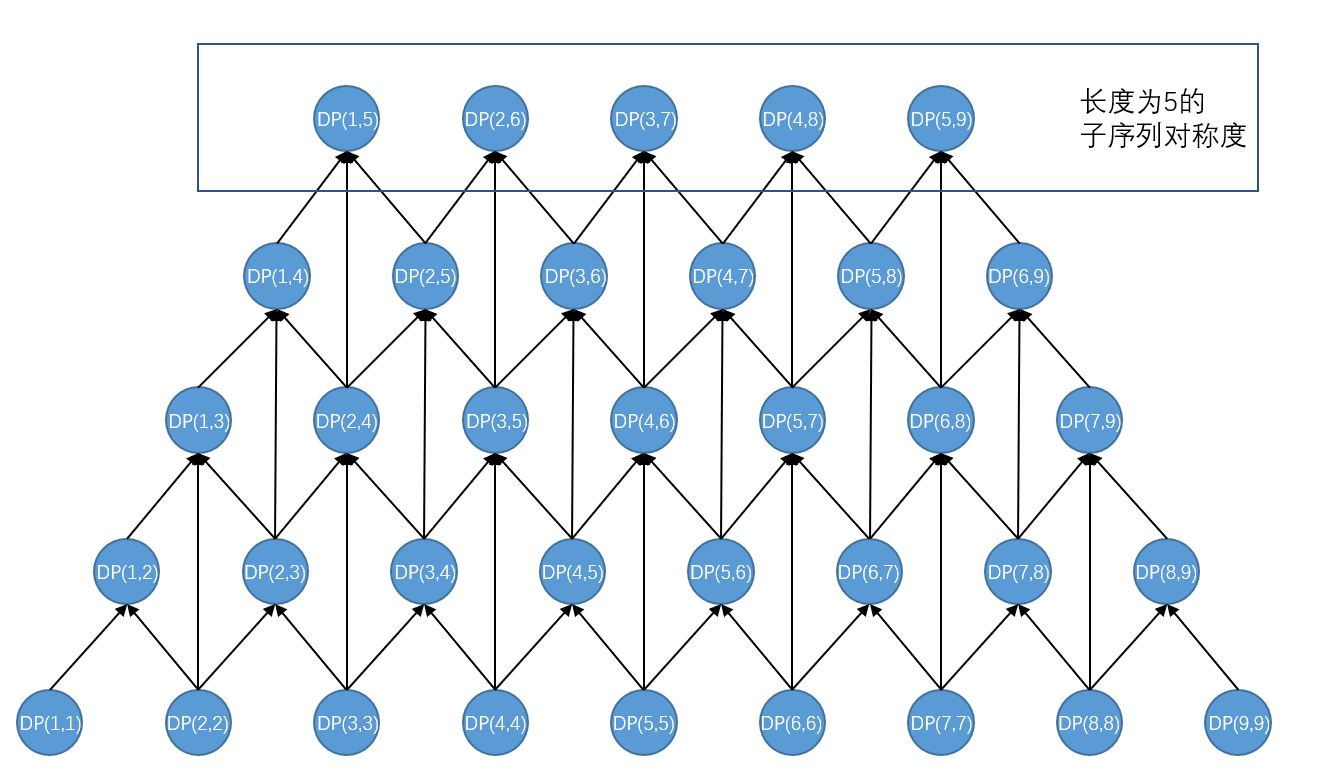
\includegraphics[width=0.76\linewidth]{fregment.png}
  \caption{分段时间序列推导流程}
  \label{fig:fregment}
\end{figure}

\section{分段对称度阈值确定算法}
4.1节讲述了分段时间序列的对称性度量算法,根据4.1节的算法,
给定时间序列X和子序列的长度约束$w$,可以在$O(|X| \times w)$的时间内
计算出所有的子序列对称度。然而,如果想判别出真正的对称时间子序列,
还需要至关重要的一步——确定对称度阈值。
图~\ref{fig:lontitude_symmetry}展示了运输车经度标准化处理后的时间序列和对应的分段对称度变化情况。
一般工业场景中,对称度阈值往往是由领域专家输入的。但是,并非所有的
应用场景中都能找到专业的领域专家。并且,如果对称度阈值提供的不合适,
将极大的影响对称模式的挖掘。因此,本节提出了一个基于时间序列数据特征
和对称度分布特征的对称度阈值计算方法。
\begin{figure}
  \centering
  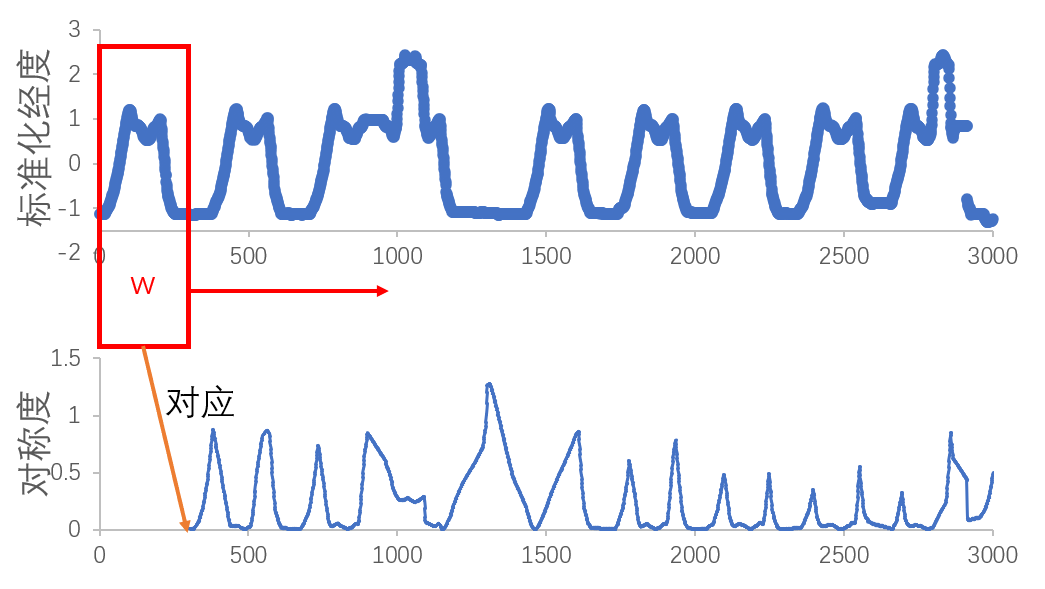
\includegraphics[width=0.76\linewidth]{std_lo_symmetry.png}
  \caption{标准化经度分段对称度变化}
  \label{fig:lontitude_symmetry}
\end{figure}

分段对称度阈值是对所有的时间子序列度量对称性,
因此,除了全局对称度阈值
考虑到的时间序列数据特征,对称度自然分布同样产生阈值划分。
基于时间序列数据特征的阈值确定算法已在3.1.2节中详述,本节只
讨论基于分布特征的对称度阈值确定算法。

在同一类时间序列中,长度相同的对称子序列的对称度较小,
而非对称子序列的对称度较大,这之间存在一个天然的阈值划分。
根据聚类方法[10]和自然断点分类的划分原则[11,12],
同一个类簇中数据的相似度高而不同类簇中数据的相似度低。
换言之,两个对称子序列的对称度差距应尽可能小,
而对称子序列与非对称子序列的对称度差距应尽可能大。
在概率统计中,方差用于衡量数据集中数据的偏离程度。
因此,很多算法使用方差作为度量指标变化的阈值[9]。
公式~\ref{eq:threshold2}展示了基于方差度量的对称度阈值确定原则,
其中,$DP_i$和$DP_j$均表示计算得到的子序列对称度,$\overline{DP_{i}}$̅和$\overline{DP_{j}}$
表示二者的均值。公式的最优化目标为在子序列对称度组成的集合中,
通过选择某个合适的值作为对称阈值,对称度小于该阈值的子序列为
对称子序列集合,对称度大于该阈值的子序列为非对称子序列集合,
使得对称子序列集合和非对称子序列集合的对称度方差之和最小。
图~\ref{fig:natural_break}展示了在运输车子序列对称度和挖掘机工况子序列对称度中
选择合适的自然断点,可使得对称模式和非对称模式的均值适中,
方差之和最小。综合时间序列数据特征和对称度分布的两类对称度阈值,
最终可以得到对称度阈值的完整公式,即式~\ref{eq:threshold}所示。
\begin{equation}
  \theta_{2}=\underset{x \in D P}{\operatorname{argmin}}\left(\sum_{D P_{i} \leq x}\left(D P_{i}-\overline{D P_{l}}\right)^{2}+\sum_{D P_{j}>x}\left(D P_{j}-\overline{D P_{j}}\right)^{2}\right)
  \label{eq:threshold2}
\end{equation}
\begin{equation}
  \theta=\min \left(\theta_{1}, \theta_{2}\right)
  \label{eq:threshold}
\end{equation}
\begin{figure}
  \centering
  \subcaptionbox{运煤车轨迹子序列对称度\label{fig:natural_break-a}}
  {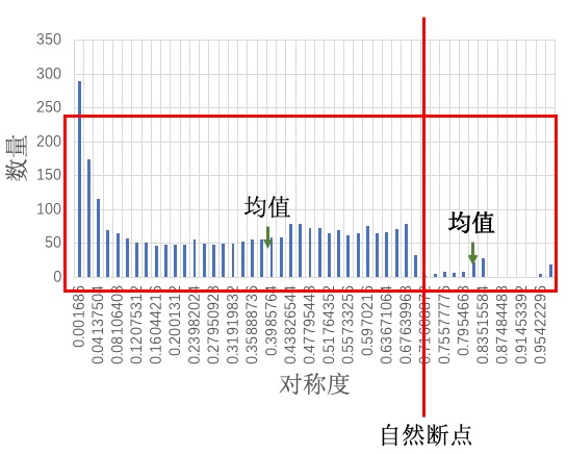
\includegraphics[width=0.42\linewidth]{natural_break-a.png}}
  \subcaptionbox{挖掘机工况子序列对称度\label{fig:natural_break-b}}
  {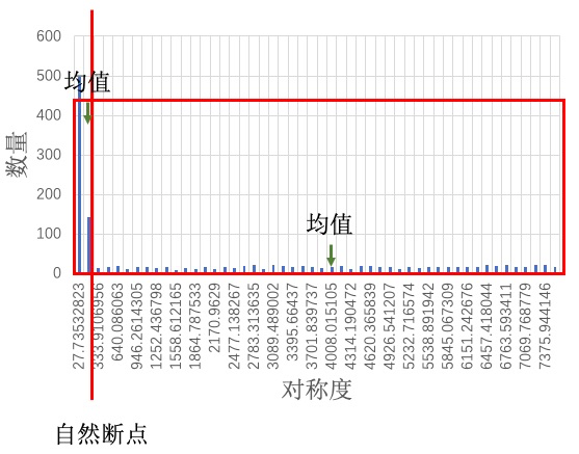
\includegraphics[width=0.42\linewidth]{natural_break-b.png}}
  \caption{运输车轨迹和挖掘机工况子序列对称度分布}
  \label{fig:natural_break}
\end{figure}

\renewcommand{\algorithmicrequire}{\textbf{输入:}\unskip}
\renewcommand{\algorithmicensure}{\textbf{输出:}\unskip}

\begin{algorithm}[t]
  \caption{对称度阈值划分算法$calculate\_threshold$}
  \label{alg:threshold}
  \small
  \begin{algorithmic}
    \REQUIRE 子序列对称度列表$y$,时间序列$X=\left(p_{1}, p_{2}, \dots, p_{n}\right)$
    \ENSURE 对称度阈值$\theta$

    \STATE sort$(y)$
    \STATE $a_1 \leftarrow y_1$
    \STATE $i \leftarrow 2$
    \WHILE{$i \leq \left|y\right|$}
    \STATE $a_i \leftarrow a_{i-1}+(y_i-a_{i-1})/{i}$
    \STATE $l_i \leftarrow (i-1) / (i \times i) \times(y_i-a_{i-1})^{2}+(i-1) / i \times l_{i-1}$
    \STATE $i \leftarrow i+1$
    \ENDWHILE

    \STATE reverse$(y)$
    \STATE $a_1 \leftarrow y_1$
    \STATE $i \leftarrow 2$
    \WHILE{$i \leq \left|y\right|$}
    \STATE $a_i \leftarrow a_{i-1}+(y_i-a_{i-1})/{i}$
    \STATE $r_i \leftarrow (i-1) / (i \times i) \times(y_i-a_{i-1})^{2}+(i-1) / i \times r_{i-1}$
    \STATE $i \leftarrow i+1$
    \ENDWHILE

    \STATE reverse$(r)$
    \STATE reverse$(y)$
    \STATE $d \leftarrow l_1 + r_2$
    \STATE $idx \leftarrow 1$
    \STATE $i \leftarrow 2$
    \WHILE{$i < \left|X\right|$}
    \IF{$l_i + r_{i+1} < d$}
    \STATE $d \leftarrow l_i + r_{i+1}$
    \STATE $idx \leftarrow i$
    \ENDIF
    \STATE $i \leftarrow i+1$
    \ENDWHILE
    \STATE $i \leftarrow 1$
    \WHILE{$i < \left|X\right|$}
    \STATE minus $\leftarrow$ minus $+D\left(p_{i}, p_{i+1}\right)$
    \STATE $i \leftarrow i+1$
    \ENDWHILE
    \STATE $\theta \leftarrow \min \left({\text { minus }} / (n-1), {dp_{idx}} / {n}\right)$
    \RETURN $\theta$
  \end{algorithmic}
\end{algorithm}

算法~\ref{alg:threshold}给出了对称度阈值的算法,考虑到
基于对称度分布的阈值确定算法需要用到
动态集合方差的计算,本文采用了流式的方差计算方法。
第1行按照大小顺序对对称度进行排序,为方差的流式计算做准备。
第2-8行根据流式算法计算前i小的对称度方差并保存到数组$l$中,从而得到
顺序排序的前缀方差数组。
第9-16行将对称度倒序排序后计算前$i$大的对称度方差并保存到数组$r$中,
由此得到倒序排序的前缀方差数组。
第17-28行通过计算前$i$小和后$n-i$大的对称度方差之和的最小值
得到基于对称度分布的阈值。
第24-35行计算时间序列相邻点距离的均值得到全局对称度阈值,
并通过和对称度分布阈值比较得到较小者,作为最终的对称度阈值。
采用这种算法得到的对称度阈值不仅考虑到了时间序列本身的特征,
还考虑到了对称度的分布,在实验结果中有良好的表现。

\section{挖掘分段对称模式}

计算出时间序列$X$所有在长度约束范围之内的子序列对称度之后,
可以利用贪心算法挖掘得到所有满足对称性的子序列。以斗杆外摆为例,
在挖掘过程中,存在对称子序列相互包含的情况。如图~\ref{fig:overlap}
中所示,子序列$a$、$b$、$c$均是对称子序列。由于要挖掘不重叠对称子序列,
若结果集合中选择了$a$,则不能再选择$b$和$c$。因此,
为了充分利用时间序列的信息,本文以对称子序列的数量最大值为
优化目标。根据贪心算法的思想,若上一个选择的对称子序列为$s_i$
其长度为$w$,则下一个对称子序列的贪心策略为从数据点$i+w$
开始,选择第1个长度为$w$的对称子序列, 可以保证能得到数量最多的
不重叠子序列。换言之,对于两个长度为$w$且存在重叠的时间序列,选择开始点最早的
时间序列能保证挖掘到数量最多的对称子序列。具体证明如下:假设存在3个长度为$w$的对称子序列
$A=\left(p_{i}, p_{i+1}, \dots, p_{i+w-1}\right)$,$B=\left(p_{j}, p_{j+1}, \dots, p_{j+w-1}\right)$和
$C=\left(p_{k}, p_{k+1}, \dots, p_{k+w-1}\right)$,并且$i<j<k$。若选择A序列进入
对称模式集合,则剩余对称模式可以从$p_{i+w}$之后的点进行选取。若选择B序列进入
对称模式集合,则剩余对称模式可以从$p_{j+w}$之后的点进行选取。由$i<j$可知,
$i+w<j+w$,前者的选择范围比后者更广,如果在选择B序列进入对称模式集合之后仍可选择C序列,
证明$j+w \leq k$,则$i+w$也$\leq k$,同样也可以选择A序列来替换B序列进入对称模式集合。
反之,如果选择A序列进入对称模式集合,则不一定可以由B序列替换。因此,对于长度相同的对称子序列,
选择起始时间点最早的序列能保证挖掘出最多的对称模式。

\begin{figure}
  \centering
  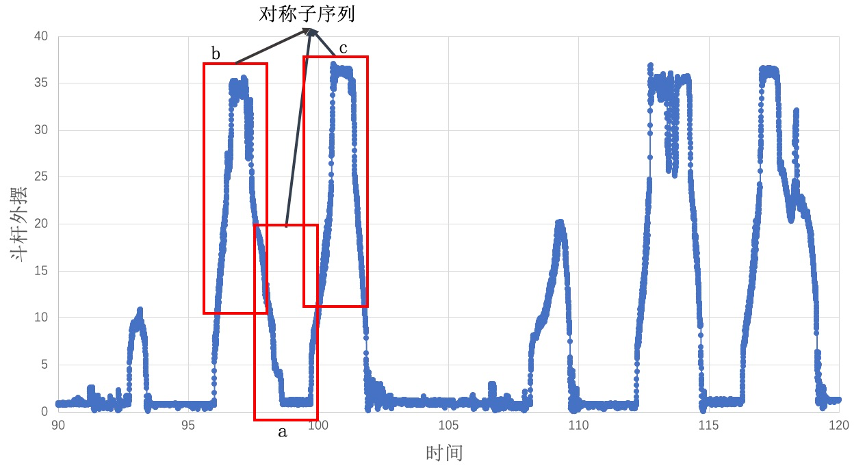
\includegraphics[width=0.80\linewidth]{symmetric_overlap.png}
  \caption{对称时间序列反映重叠现象的案例}
  \label{fig:overlap}
\end{figure}

本文根据上述对称模式挖掘方法提出了相应的具体算法,
如算法3.2所示。第1-19行根据第3.2节提出的对称度计算方式
计算了给定时间长度约束下所有子序列的对称度,第20行根据算法~\ref{alg:threshold}的计算方式
确定了对称度阈值,第21-30行根据贪心策略
计算出数量最多的不重叠对称子序列。由前述定义可知,第1-19行计算子序列对称度的时间复杂度为$O(|X| \times w)$,
第20行自然断点的确定和不重叠对称子序列的挖掘均只需要$O(|X|)$的时间。
因此,本算法的整体时间复杂度为$O(|X| \times w)$,其效率远远高于直接利用
DTW 计算的$O\left(|X| \times w^{2}\right)$,为后续的数据分析提供数据基础。
\renewcommand{\algorithmicrequire}{\textbf{输入:}\unskip}
\renewcommand{\algorithmicensure}{\textbf{输出:}\unskip}

\begin{algorithm}
  \caption{时间序列对称模式挖掘算法$calculate\_symmtric\_pattern$}
  \label{alg:symmetric_pattern}
  \small
  \begin{algorithmic}
    \REQUIRE 时间序列$X=\left(p_{1}, p_{2}, \dots, p_{n}\right)$,长度约束$w$
    \ENSURE 对称模式$Q$

    \STATE $i \leftarrow 1$
    \WHILE{$i \leq \left|X\right|$}
    \STATE $dp_{i,i} \leftarrow inf$
    \ENDWHILE

    \STATE $i \leftarrow 1$
    \WHILE{$i < \left|X\right|$}
    \STATE $dp_{i,i+1} \leftarrow D\left(p_{i}, p_{i+1}\right)$
    \ENDWHILE

    \STATE $len \leftarrow 3$
    \WHILE{$len \leq \left|X\right|$}
    \STATE $i \leftarrow len$
    \WHILE{$i \leq \left|X\right|-len+1$}
    \STATE $dp_{i,i+len-1} = D\left(p_{i}, p_{i+1}\right)+\min \left(dp_{i,i+len-2},dp_{i+1,i+len-1},dp_{i+1,i+len-2}\right)$
    \ENDWHILE
    \ENDWHILE

    \STATE $i \leftarrow 1$
    \WHILE{$i \leq \left|X\right|-w+1$}
    \STATE $y_i=dp_{i,i+w-1}$
    \ENDWHILE
    \STATE $\theta = calculate\_threshold\left(y,X\right)$

    \STATE $i \leftarrow 1$
    \WHILE{$i \leq \left|X\right|-w+1$}
    \IF{$dp_{i,i+w-1}/w \leq \theta$}
    \STATE 把$S=\left(p_{i+1}, p_{i+2}, \dots, p_{i+w-1}\right)$放入对称子序列集合$Q$
    \STATE $i \leftarrow i+w$
    \ELSE
    \STATE $i \leftarrow i+1$
    \ENDIF
    \ENDWHILE
    \RETURN $Q$
  \end{algorithmic}
\end{algorithm}

\section{基于IoTDB的分段对称模式挖掘算法设计}

Apache IoTDB是面向时间序列的原生数据库,是一个集
数据收集、存储和分析于一体的数据管理引擎,不仅提供了类SQL
的数据查询功能,而且预留了基于原生接口和UDF(User Defined 
Function)接口的数据分析功能,具有高度的可扩展性。本节将利用
IoTDB提供的数据分析接口设计并优化分段对称模式挖掘算法。







% \section{自适应窗口的设计与实现}
% 时间序列的数据和模式均具有很强的随机性,同一个时间序列中的
% 对称模式其数据点个数可能不严格相等,而是处于某个合理范围之内。
% 以挖掘机为例,挖掘不同的坑道时,斗杆移动的轨迹就不同。
% 当对称模式长度约束设置得较大时,长度较小的模式则挖掘不出。
% 而当人为设置长度约束为所有对称模式的最小长度时,
% 尽管可以保证挖掘出长度较小的对称模式,
% 但是较长模式的信息却经常存在缺失,影响算法挖掘结果的完整性。
% 图~\ref{fig:excavator_diff_route}展示了挖掘机在不同坑道
% 挖掘作业斗杆外摆工况变化时间序列。若设定对称子序列的数据点个数
% 即窗口长度为坑道a的序列长度,则坑道b的对称子序列不能完全挖掘。
% 因此,当需要挖掘的
% 对称模式长度不一时,窗口需要在原始长度约束大小上进行自适应的变化
% 以挖掘出完整的对称模式。本节利用数据点差分的分布特征,
% 设计了一种自动调节大小的窗口算法。

% 根据时间序列对称性的定义,在设定对称子序列的长度$w$之后,
% 挖掘出的对称时间子序列$X=\left(p_{i},p_{i+2},…,p_{i+w-1} \right)$
% 的首尾点$p_{i}$和$p_{i+w-1}$必定匹配。
% 换言之,首尾点的距离若接近0,
% 则证明该窗口大小合适;若远大于0,则证明需调大窗口,
% 以完整获取对称子序列的全部信息。
% 因此,可以使用时间子序列首尾点的距离来衡量窗口大小设置得
% 是否合适。
% \begin{figure}
%   \centering
%   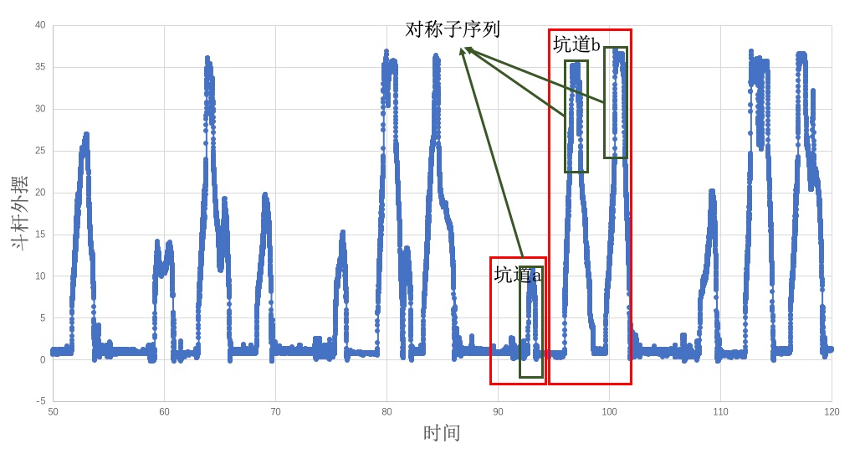
\includegraphics[width=0.86\linewidth]{excavator_diff_route.png}
%   \caption{挖掘机在不同坑道挖掘作业斗杆外摆工况时间序列}
%   \label{fig:excavator_diff_route}
% \end{figure}

% 然而,真实工业场景中的匹配数据点往往具有误差,
% 并不一定满足首尾点距离为0。因此,本文考虑利用相邻点距离
% 所组成数据集的分布特点,判断窗口是否应当扩张。
% 根据工业大数据时间序列点的随机性,首尾数据点的距离所组成的
% 数据集应满足正态分布的特点[13],且其均值为0。也就是说,
% 若一个窗口内的相邻点距离集合为
% $s=\left\{D\left(p_{1}, p_{2}\right), D\left(p_{2}, p_{3}\right), \ldots, D\left(p_{n-1}, p_{n}\right)\right\}$,
% 则首尾数据点距离的应满足均值为$\mu=0$且标准差$\sigma=\sigma_s$
% 的正态分布。按照3$\sigma$原则,首尾数据点的距离应在
% $\left[0,3\sigma\right]$范围之内。

% 此外,考虑到相邻点的距离属于差分计算。
% 因此,相比标准差,绝对中位差更加适合度量
% 相邻点距离集合的分布差异。
% 绝对中位差指的是所有元素与其中位数的偏差的绝对值,
% 相比标准差具有更强的鲁棒性,
% 且已有较为成熟的近似算法加快计算[14]。因此,本节使用窗口内
% 相邻数据点的距离绝对中位差作为$\sigma$,
% 首尾点的距离应在$\left[0,3\sigma\right]$之间。
% 指定窗口的基础长度约束$w_{base}$和最长长度约束$w_{max}$,
% 若窗口的终点和起点的距离
% 在$\left[0,3\sigma\right]$范围之内,则窗口闭合。
% 否则,则继续调大窗口,直到窗口大小为$w_{max}$为止。
% 具体的计算流程如算法~\ref{alg:adaptive_window}所示。

% \renewcommand{\algorithmicrequire}{\textbf{输入:}\unskip}
% \renewcommand{\algorithmicensure}{\textbf{输出:}\unskip}

% \begin{algorithm}[h]
%   \caption{自适应窗口算法$adaptive\_window$}
%   \label{alg:adaptive_window}
%   \small
%   \begin{algorithmic}
%     \REQUIRE 时间序列$X=\left(p_1,p_2,…,p_n\right)$,基础模式长度$w_{base}$,最长模式长度$w_{max}$
%     \ENSURE 调整后的窗口大小$t$

%     \STATE $\sigma=\operatorname{mad}(X, w_{max})$
%     \STATE $t \leftarrow w_{base}$
%     \STATE $i \leftarrow 1$
%     \WHILE{$i+t<|X| \& \& t<w_{max} \& \& D\left(p_{i}, p_{i+1}\right)>3 \sigma$}
%       \STATE $t \leftarrow t+1$
%     \ENDWHILE
%     \RETURN $t$
%   \end{algorithmic}
% \end{algorithm}

\section{本章小结}
本章主要介绍了时间序列对称模式挖掘在更多应用场景下的扩展。
首先,流式时间序列数据作为一种在工业和金融领域经常出现的数据
类型,对其进行对称模式挖掘具有重要的研究价值。但是,
度量所有时间子序列的对称性会产生大量重复计算,时间效率低,
且对称度阈值也不好判定。本章根据全局时间序列对称模式挖掘算法
的状态推导方式,在对称度矩阵上创造性地引入了滑动窗口,
在不违反对称度状态连续性和单调性的前提下,采用以空间换时间的
策略将流式对称模式的计算时间复杂度由$O\left(w^2\right)$
提升至了$O\left(w\right)$。
此外,为了在时间序列中挖掘完整的对称模式,本章还在对称模式的
挖掘过程中引入了自适应窗口,通过时间序列的数据特征自动地调节
窗口大小,以保证挖掘对称模式的完整性。对称模式挖掘在不同的
应用中具有很好的可扩展性,通过设置不同的约束可以灵活地调整
对称模式挖掘算法,从而满足不同场景的需要。

% 模板支持 BibTeX 和 BibLaTeX 两种方式处理参考文献。
% 下文主要介绍 BibTeX 配合 \pkg{natbib} 宏包的主要使用方法。


% \section{顺序编码制}

% 在顺序编码制下,默认的 \cs{cite} 命令同 \cs{citep} 一样,序号置于方括号中,
% 引文页码会放在括号外。
% 统一处引用的连续序号会自动用短横线连接。

% \thusetup{
%   cite-style = super,
% }
% \begin{tabular}{l@{\quad$\Rightarrow$\quad}l}
%   \verb|\cite{zhangkun1994}|               & \cite{zhangkun1994}               \\
%   \verb|\citet{zhangkun1994}|              & \citet{zhangkun1994}              \\
%   \verb|\citep{zhangkun1994}|              & \citep{zhangkun1994}              \\
%   \verb|\cite[42]{zhangkun1994}|           & \cite[42]{zhangkun1994}           \\
%   \verb|\cite{zhangkun1994,zhukezhen1973}| & \cite{zhangkun1994,zhukezhen1973} \\
% \end{tabular}


% 也可以取消上标格式,将数字序号作为文字的一部分。
% 建议全文统一使用相同的格式。

% \thusetup{
%   cite-style = inline,
% }
% \begin{tabular}{l@{\quad$\Rightarrow$\quad}l}
%   \verb|\cite{zhangkun1994}|               & \cite{zhangkun1994}               \\
%   \verb|\citet{zhangkun1994}|              & \citet{zhangkun1994}              \\
%   \verb|\citep{zhangkun1994}|              & \citep{zhangkun1994}              \\
%   \verb|\cite[42]{zhangkun1994}|           & \cite[42]{zhangkun1994}           \\
%   \verb|\cite{zhangkun1994,zhukezhen1973}| & \cite{zhangkun1994,zhukezhen1973} \\
% \end{tabular}



% \section{著者-出版年制}

% 著者-出版年制下的 \cs{cite} 跟 \cs{citet} 一样。

% \thusetup{
%   cite-style = author-year,
% }
% \begin{tabular}{l@{\space$\Rightarrow$\space}l}
%   \verb|\cite{zhangkun1994}|                & \cite{zhangkun1994}                \\
%   \verb|\citet{zhangkun1994}|               & \citet{zhangkun1994}               \\
%   \verb|\citep{zhangkun1994}|               & \citep{zhangkun1994}               \\
%   \verb|\cite[42]{zhangkun1994}|            & \cite[42]{zhangkun1994}            \\
%   \verb|\citep{zhangkun1994,zhukezhen1973}| & \citep{zhangkun1994,zhukezhen1973} \\
% \end{tabular}

% \vskip 2ex
% \thusetup{
%   cite-style = super,
% }
% 注意,引文参考文献的每条都要在正文中标注
% \cite{zhangkun1994,zhukezhen1973,dupont1974bone,zhengkaiqing1987,%
%   jiangxizhou1980,jianduju1994,merkt1995rotational,mellinger1996laser,%
%   bixon1996dynamics,mahui1995,carlson1981two,taylor1983scanning,%
%   taylor1981study,shimizu1983laser,atkinson1982experimental,%
%   kusch1975perturbations,guangxi1993,huosini1989guwu,wangfuzhi1865songlun,%
%   zhaoyaodong1998xinshidai,biaozhunhua2002tushu,chubanzhuanye2004,%
%   who1970factors,peebles2001probability,baishunong1998zhiwu,%
%   weinstein1974pathogenic,hanjiren1985lun,dizhi1936dizhi,%
%   tushuguan1957tushuguanxue,aaas1883science,fugang2000fengsha,%
%   xiaoyu2001chubanye,oclc2000about,scitor2000project%
% }。
